%%=============================================================================
%% Methodologie
%%=============================================================================

\chapter{\IfLanguageName{dutch}{Methodologie}{Methodology}}%
\label{ch:methodologie}

%% TODO: In dit hoofstuk geef je een korte toelichting over hoe je te werk bent
%% gegaan. Verdeel je onderzoek in grote fasen, en licht in elke fase toe wat
%% de doelstelling was, welke deliverables daar uit gekomen zijn, en welke
%% onderzoeksmethoden je daarbij toegepast hebt. Verantwoord waarom je
%% op deze manier te werk gegaan bent.
%%
%% Voorbeelden van zulke fasen zijn: literatuurstudie, opstellen van een
%% requirements-analyse, opstellen long-list (bij vergelijkende studie),
%% selectie van geschikte tools (bij vergelijkende studie, "short-list"),
%% opzetten testopstelling/PoC, uitvoeren testen en verzamelen
%% van resultaten, analyse van resultaten, ...
%%
%% !!!!! LET OP !!!!!
%%
%% Het is uitdrukkelijk NIET de bedoeling dat je het grootste deel van de corpus
%% van je bachelorproef in dit hoofstuk verwerkt! Dit hoofdstuk is eerder een
%% kort overzicht van je plan van aanpak.
%%
%% Maak voor elke fase (behalve het literatuuronderzoek) een NIEUW HOOFDSTUK aan
%% en geef het een gepaste titel.

This section contains a brief description of the road map to build the proof of concept (PoC), which combines the general key insights from the literature.

The proposed model can be seen as a three-way modular setup. Each step can be improved individually in order to acquire the best possible result and is implemented independently.
The first step focuses on localizing the athletes in the field in order to crop them out and spare computational resources. Next up is segmenting each skill performed in a given routine. The final part involves recognizing each isolated skill.

% TODO : chart overview of model.

\section{Genral information}

Before jumping into each different step, some general information is provided. Each of the 458 DD3 freestyles collected, 2231 in total. Each video has a record in the database. Two selections have been made to decide the videos in the validation set. The first selection is filtering all videos of this season (67 videos). The second selection uses the id of the video. In the beginning of the project, taking the 10th modulo of the id being 5 resulted in the most validation videos. Currently this corresponds to 42 validation videos. The other 90\% are used as training videos (349).
Each recording lasts for about 60 to 75 seconds, depending on the competition level and has around 40 to 60 performed skills. These do not include normal jumps. In order to annotate the videos, a custom Vue3 web application is created. In order to render the videos in the browsers, conversions from blu-ray (m2ts) or AVI to mp4 were required. Most videos have a framerate of 25, 30 or 50 frames per second (fps), while some may be 15, 28 or 60.
The quality of videos differ and range from anywhere between 8 and 550MB. It may not indicate much, but just to keep in mind. Even on the more qualitative videos, the rope disappears when making quick rotations. This is often better on higher fps videos.

\section{Jumper localization}
\label{methodology:jumper-localization}

Jumper localization is needed in order crop a zoomed-in video of the skippers performing their routine. Image \ref{fig:sr4-field} perfectly illustrates a competition setting, where the majority of the video is lost on surroundings, judges and spectators.

For predicting the location of the athletes, any object detection model is fine with slight preference towards a model like YOLO or EfficientDet having a higher FPS rate than others based on survey of \textcite{Zaidi_2021}. In order to compare which model is suited for next steps, the Jaccard similarity coefficient, or intersection over union is used. 
Using the predicted locations of the skippers, each frame of video can be cropped around the athletes.

Potential obstacles are predicted spectators or blurry athletes mid-skill being unrecognizable. Refer to the result chapter~\ref{ch:results} for more details on the solution.

\begin{figure}
    \centering
    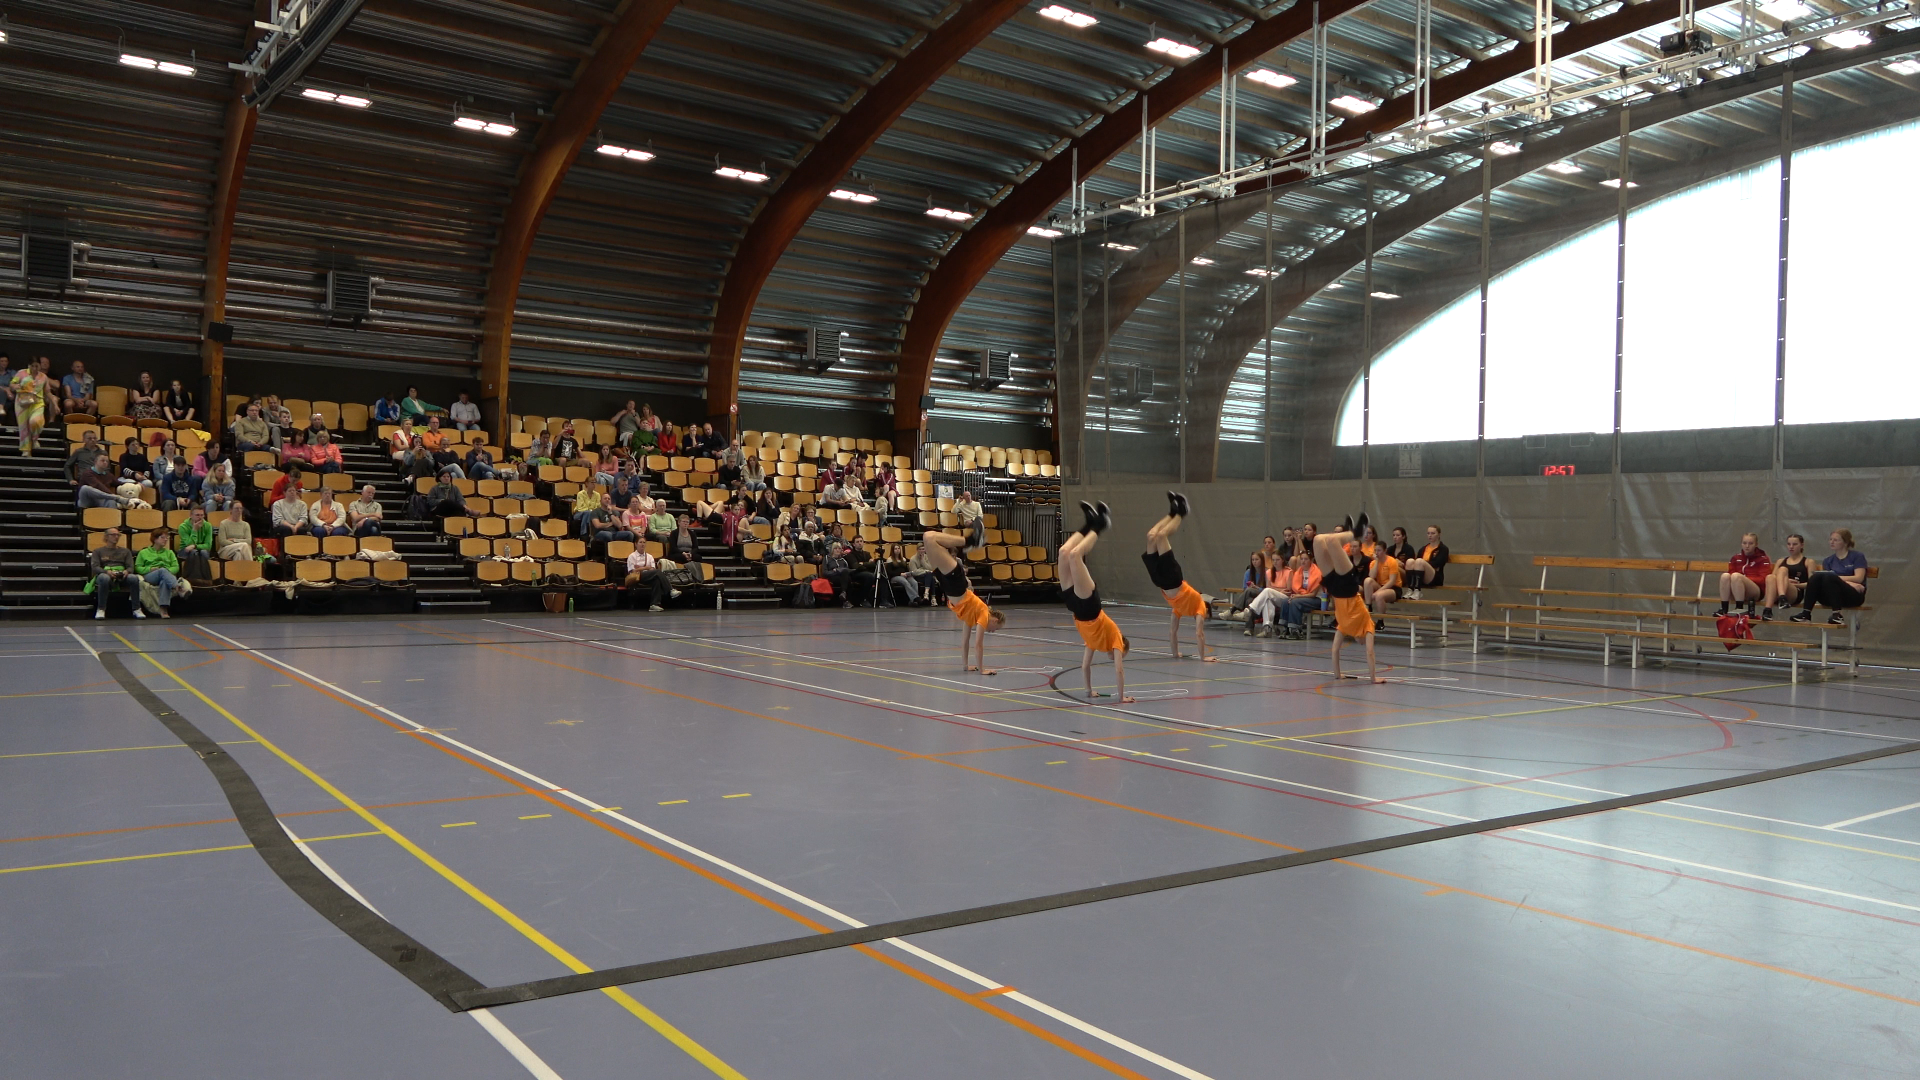
\includegraphics[width=0.95\linewidth]{sr4-field}
    \caption[Example jump rope competition setting]{Example of a competition setting in which four athletes are performing a SR4 freestyle.}
    \label{fig:sr4-field}
\end{figure}


\section{Action segmentation}
\label{methodology:action-segmentation}

The main purpose of the action segmentation is to enable predictions on full routines in order to actually use the whole model. Using the cropped images, and the assigned start and end frame of a skill, the model can predict whether a given frame is an interesting split point or not.

For jump rope, this mostly means moments when an athlete leaves or lands on the floor. However there are special cases such as cartwheels. Only moments when either hands or feet land over a rope, are annotated as the end of a skill. A couple of models can be tried as the idea of leaving and landing on the floor seems relatively straightforward. This means more simple convolutional models to models incorporating temporal information.
The best model or an ensemble of the best ones will be used in the full sequence.

A couple of ideas exist in order mark interesting split moments. Both the frame before and the frame after each split point can be assigned as split point, selecting the one with the highest probability as the final split point. Another idea would be to assign higher values to split points using a cyclic function like the sinus depending on its distance between two split points.

\section{Skill recognition}
\label{methodology:skill-recognition}

The last part involves recognizing the performed skill, which is, as introduced in the literature, a combination of different aspects. What are the turners doing, using one or both arms, an additional body rotation, etc.
For this part, a video vision model is definitely required to fill in the temporal information, e.g. amount of rotations.
Along the way, additional aspects to a skill label can be added in order to incorporate for every level and skill variation.
Furthermore, once-in-a-lifetime skills can be marked as unknown in order for the model to be robust in predicting new skills. After analyzing the given skillsection, a level can be assigned, based on the predicted aspects.
Multiple different models can be tested in order to find the best one.


\section{Judge score comparison}
\label{methodology:judge-score-comparison}

Finally, when skills are predictable, a comparison between the jury assigned scores, the models prediction and the effective score can be made in order to check whether model predictions could be used or more research/training is needed. This is an additional check, beside the accuracy of the model or confusion matrices.

